\documentclass{article}
\usepackage{amsmath}
\usepackage{titlesec}
\usepackage{graphicx}
\usepackage[margin=1in]{geometry}
\usepackage{hyperref}
\usepackage{amssymb}
\usepackage{bm}


% Title, date, and author
\title{Exercise 4}
\author{Your Name, Collaborator's Name}
\date{\today}

\titleformat{\section}
  {\normalfont\normalsize\bfseries} % Format: font style, size, and weight
  {\thesection}{1em} % Label format and spacing
  {}
  \renewcommand{\thesubsection}{\thesection.\alph{subsection}}

\titleformat{\subsection}
  {\normalfont\small\bfseries} % Format: font style, size, and weight
  {\thesubsection}{1em} % Label format and spacing
  {}
\titleformat{\subsubsection}
  {\normalfont\small\bfseries} % Format: font style, size, and weight
  {\thesubsubsection}{1em} % Label format and spacing
  {}

\begin{document}
\begin{titlepage}
    \centering
    \vspace*{1in}
    
    {\Huge\bfseries Exercise 4\par}
    \vspace{1.5cm}
    {\Large \today\par}
    \vspace{1.5cm}
    {\Large\itshape Antonio Pampalone 23586519 \\ Giuseppe Pisante 23610012\\ Martina Raffaelli 23616907 \par}
    
    \vfill
    
\includegraphics[width=0.3\textwidth]{FAU-Logo.png}\par\vspace{1cm} % Adjust the width as needed
   
\end{titlepage}

\newpage
\small

\section{Stability of the unsteady advection-diffusion equation}

\subsection{Discretization of of the unsteady one-dimensional advection-diffusion equation}


We start with the one-dimensional advection-diffusion equation:

\[
\rho \left( \frac{\partial \Phi}{\partial t} + U \frac{\partial \Phi}{\partial x} \right) = \alpha \frac{\partial^2 \Phi}{\partial x^2}.
\]

We use central finite differencing in space and explicit Euler in time. The terms are discretized as follows:

\begin{itemize}
    \item \(\frac{\partial \Phi}{\partial t} \approx \frac{\Phi_i^{n+1} - \Phi_i^n}{\Delta t}\)
    \item \(\frac{\partial \Phi}{\partial x} \approx \frac{\Phi_{i+1}^n - \Phi_{i-1}^n}{2\Delta x}\)
    \item \(\frac{\partial^2 \Phi}{\partial x^2} \approx \frac{\Phi_{i+1}^n - 2\Phi_i^n + \Phi_{i-1}^n}{\Delta x^2}\)
\end{itemize}

Substituting these approximations into the original equation, we get:

\[
\rho \left( \frac{\Phi_i^{n+1} - \Phi_i^n}{\Delta t} \right) + \rho U \left( \frac{\Phi_{i+1}^n - \Phi_{i-1}^n}{2\Delta x} \right) = \alpha \left( \frac{\Phi_{i+1}^n - 2\Phi_i^n + \Phi_{i-1}^n}{\Delta x^2} \right).
\]

Multiplying through by \(\Delta t\):

\[
\rho \Phi_i^{n+1} - \rho \Phi_i^n + \rho U \Delta t \left( \frac{\Phi_{i+1}^n - \Phi_{i-1}^n}{2\Delta x} \right) = \alpha \Delta t \left( \frac{\Phi_{i+1}^n - 2\Phi_i^n + \Phi_{i-1}^n}{\Delta x^2} \right).
\]

Rearranging to isolate \(\Phi_i^{n+1}\) on the left-hand side:

\[
\rho \Phi_i^{n+1} = \rho \Phi_i^n - \rho U \Delta t \left( \frac{\Phi_{i+1}^n - \Phi_{i-1}^n}{2\Delta x} \right) + \alpha \Delta t \left( \frac{\Phi_{i+1}^n - 2\Phi_i^n + \Phi_{i-1}^n}{\Delta x^2} \right).
\]

Dividing through by \(\rho\):

\begin{equation}
  \label{eq:discretized}
\Phi_i^{n+1} = \Phi_i^n - c \left( \frac{\Phi_{i+1}^n - \Phi_{i-1}^n}{2} \right) + d \left( \Phi_{i+1}^n - 2\Phi_i^n + \Phi_{i-1}^n \right),
\end{equation}

where:

\[
c = \frac{U \Delta t}{\Delta x}, \quad d = \frac{\alpha \Delta t}{\rho (\Delta x)^2}.
\]

The parameter $c$ represents the Courant number and quantifies the influence of advection in the simulation. 
For stability and accuracy in explicit schemes, $c$ should typically be small to satisfy the Courant-Friedrichs-Lewy condition that requires $c \leq 1$. 
If $c$ is too large, the simulation may become unstable or inaccurate because the flow travels across more than one grid cell per time step.
The parameter $d$ measures the contribution of diffusion to the simulation and it should typically be small to ensure numerical stability.
The diffusion stability condition generally requires $d \leq 1/2$ to ensure that diffusion does not dominate excessively or destabilize the solution.


\subsection{Stability Analysis Using Von Neumann Method}
Given the discretized convection-diffusion equation \eqref{eq:discretized}, we can perform a Von Neumann stability analysis to determine the stability conditions for the explicit scheme. 
\\This is made possible due to the linear nature of such equation and by not considering the imact of boundary conditions. 
We will consider the domain as periodic in \(x\), allowing the solution and the error to be expressed using a Fourier series with a period of length \(2L\).

Assuming a disturbance of the form:

\[
\epsilon(x, t) = V(t) e^{ikx},
\]

where $\theta = k \Delta x$ is the phase angle.
\\We can insert the error function \(epsilon(x, t)\) into the discretized differential equation and estimate the temporal behaviour of the amplitude by evaluation the amplification factor \(G\). This can be directly applied to the solution, by exploiting the linearity of the equation so that:

\[
\phi_i^n = V^n e^{I \theta i}, \quad \phi_{i+1}^n = V^n e^{I \theta (i+1)}, \quad \phi_{i-1}^n = V^n e^{I \theta (i-1)}.
\]

Substituting into the discretized equation:

\[
V^{n+1} = V^n \left(1 - \frac{c}{2} (e^{I \theta} - e^{-I \theta}) + d (e^{I \theta} - 2 + e^{-I \theta})\right).
\]

By considering the Euler relation \(e^{I \theta} = \cos \theta + I \sin \theta\), we can simplify the equation to:

\[
V^{n+1} = V^n \left(1 - I c \sin \theta + 2d (\cos \theta - 1)\right).
\]

The amplification factor $G$, which can be computed for subsequent steps, is the following:

\[
G = 1 - i c \sin \theta + 2d (\cos \theta - 1).
\]

To obtain stability, by remembering that the amplification factor should damp the error to obtain stability, we require that the absolute value of $G$ is less than or equal to 1:

\[
|G| \leq 1.
\]

We then compute $|G|^2$ to find the stability condition on the real domain:

\[
|G|^2 = \left(1 + 2d (\cos \theta - 1)\right)^2 + (c \sin \theta)^2.
\]

For stability, we need to find the values of $c$ and $d$ that satisfy the condition:

\[
|G|^2 \leq 1.
\]

We can solve this with variable substitution and trigonometric identities to find the stability condition for the explicit scheme.
We get the following disequation:

\[
t^2(1-\frac{c^2}{4d^2}) + t(\frac{1}{d}-2) + 1 (1-\frac{1}{d}+\frac{c^2}{4d^2}) \leq 0.,
\]

where \(t = \cos \theta\).

We can thus solve it by applying the general quadratic formula to find the stability condition:

\begin{equation}
\frac{\frac{1}{d}-2-\sqrt{(\frac{1}{d}-2)^2-4(1-\frac{c^2}{4d^2})(1-\frac{1}{d}-\frac{c^2}{4d^2})}}{2(1-\frac{c^2}{4d^2})}\leq t
\end{equation}
\begin{equation}
t \leq \frac{\frac{1}{d}-2+\sqrt{(\frac{1}{d}-2)^2-4(1-\frac{c^2}{4d^2})(1-\frac{1}{d}-\frac{c^2}{4d^2})}}{2(1-\frac{c^2}{4d^2})}
\end{equation}

We can now substitute the values of \(c\) and \(d\) to find the stability condition for the explicit scheme.
We recall that \(c\)=\(\frac{U \Delta t}{\Delta x}\) and \(d\)=\(\frac{\alpha \Delta t}{\rho (\Delta x)^2}\).

By substituting this in the disequation we get:

\begin{equation}
\frac{\frac{\alpha \Delta t}{\rho (\Delta x)^2}-2-\sqrt{(\frac{\alpha \Delta t}{\rho (\Delta x)^2}-2)^2-4(1-\frac{U^2 \Delta t^2}{4 \alpha \Delta x^2})(1-\frac{\alpha \Delta t}{\rho (\Delta x)^2}-\frac{U^2 \Delta t^2}{4 \alpha \Delta x^2})}}{2(1-\frac{U^2 \Delta t^2}{4 \alpha \Delta x^2})}\leq t
\end{equation}
\begin{equation}
  t \leq \frac{\frac{\alpha \Delta t}{\rho (\Delta x)^2}-2+\sqrt{(\frac{\alpha \Delta t}{\rho (\Delta x)^2}-2)^2-4(1-\frac{U^2 \Delta t^2}{4 \alpha \Delta x^2})(1-\frac{\alpha \Delta t}{\rho (\Delta x)^2}-\frac{U^2 \Delta t^2}{4 \alpha \Delta x^2})}}{2(1-\frac{U^2 \Delta t^2}{4 \alpha \Delta x^2})}
\end{equation}
Given the complexity of the disequation, it is beneficial to analyze the two extreme cases: \(\theta = 0\) and \(\theta = \pi\).

\begin{enumerate}
  \item \textbf{Case 1: \( \theta = \pi \) (Maximum Frequency)}

  At \( \theta = \pi \), we have:

  \[
  \cos \pi = -1, \quad \sin \pi = 0.
  \]

  Substitute into the expression for \( G \):

  \[
  G = 1 + 2d (-1 - 1) = 1 - 4d.
  \]

  The magnitude is:

  \[
  |G|^2 = (1 - 4d)^2.
  \]

  For instability, we need:

  \[
  (1 - 4d)^2 > 1.
  \]

  Taking the square root:

  \[
  |1 - 4d| > 1.
  \]

  This gives two conditions:

  \[
  1 - 4d > 1 \quad \text{or} \quad 1 - 4d < -1.
  \]

  Solving these inequalities:

  \begin{enumerate}
    \item \( 1 - 4d > 1 \implies d < 0 \) (not physically meaningful),
    \item \( 1 - 4d < -1 \implies d > \frac{1}{2} \).
  \end{enumerate}

  Thus, \textbf{instability occurs at \( \theta = \pi \) when \( d > \frac{1}{2} \)}.
  Substituting \( d = \frac{\alpha \Delta t}{\rho (\Delta x)^2} \) into the instability condition \( d > \frac{1}{2} \):

  \[
  \frac{\alpha \Delta t}{\rho (\Delta x)^2} > \frac{1}{2}.
  \]

  Rearranging to find the relationship between \( \Delta x \) and \( \Delta t \):

  \[
  \Delta t < \frac{\rho (\Delta x)^2}{2 \alpha}.
  \]

  This inequality provides the stability condition for the explicit scheme in terms of the time step \( \Delta t \) and the spatial step \( \Delta x \). For the scheme to be stable, the time step must be sufficiently small relative to the square of the spatial step.

  \item \textbf{Case 2: \( \theta \approx 0 \) (Low Frequencies)}

  For small \( \theta \), we use the Taylor expansions:

  \[
  \sin \theta \approx \theta, \quad \cos \theta \approx 1 - \frac{\theta^2}{2}.
  \]

  Substitute into the expression for \( G \):

  \[
  G \approx 1 - d \theta^2 - i c \theta.
  \]

  Compute \( |G|^2 \):

  \[
  |G|^2 \approx (1 - d \theta^2)^2 + (c \theta)^2.
  \]

  Neglecting terms of order \( \theta^4 \), we get:

  \[
  |G|^2 \approx 1 - 2d \theta^2 + c^2 \theta^2.
  \]

  For instability, we need:

  \[
  1 - 2d \theta^2 + c^2 \theta^2 > 1.
  \]

  Canceling the 1:

  \[
  -2d \theta^2 + c^2 \theta^2 > 0,
  \]

  or:

  \[
  (c^2 - 2d) \theta^2 > 0.
  \]

  For instability, this implies:

  \[
  c^2 > 2d.
  \]
  Substituting \( c = \frac{U \Delta t}{\Delta x} \) and \( d = \frac{\alpha \Delta t}{\rho (\Delta x)^2} \) into the instability condition \( c^2 > 2d \):

  \[
  \left( \frac{U \Delta t}{\Delta x} \right)^2 > 2 \left( \frac{\alpha \Delta t}{\rho (\Delta x)^2} \right).
  \]

  Simplifying:

  \[
  \frac{U^2 (\Delta t)^2}{(\Delta x)^2} > \frac{2 \alpha \Delta t}{\rho (\Delta x)^2}.
  \]

  Multiplying both sides by \( (\Delta x)^2 \):

  \[
  U^2 (\Delta t)^2 > \frac{2 \alpha \Delta t}{\rho}.
  \]

  Dividing both sides by \( \Delta t \):

  \[
  U^2 \Delta t > \frac{2 \alpha}{\rho}.
  \]

  Rearranging to find the relationship between \( \Delta x \) and \( \Delta t \):

  \[
  \Delta t < \frac{2 \alpha}{\rho U^2}.
  \]

  Thus, the stability condition for the explicit scheme, considering both advection and diffusion, is:

  \[
  \Delta t < \min \left( \frac{\rho (\Delta x)^2}{2 \alpha}, \frac{2 \alpha}{\rho U^2} \right).
  \]
\end{enumerate}

\section{Stability region}
\begin{figure}[h]
  \centering
  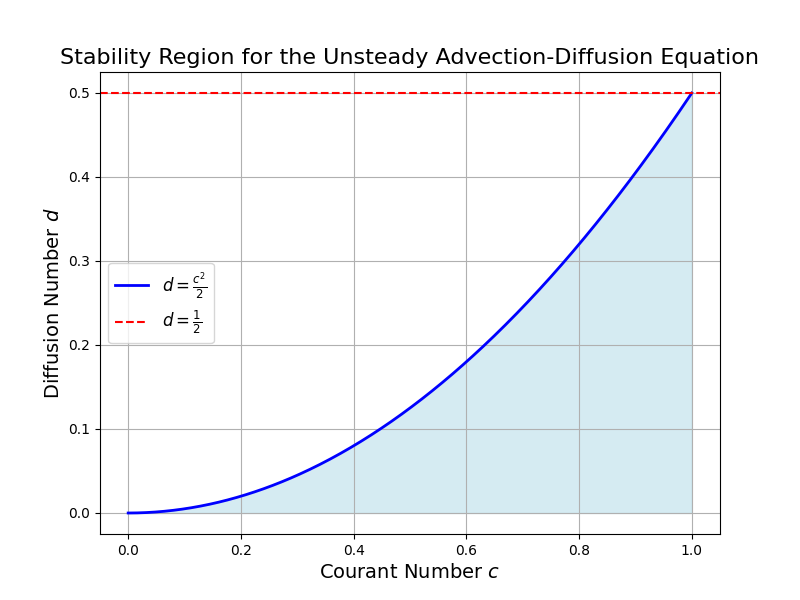
\includegraphics[width=0.8\textwidth]{stability_region_plot.png}
  \caption{Stability region for the explicit scheme.}
  \label{fig:stability_region}
\end{figure}
\begin{thebibliography}{9}
  \bibitem{GitHubRepo}
  \textit{CFD Repository},\\
  Available at: \url{https://github.com/GiuseppePisante/CFD.git}
  
  \bibitem{GitHubCopilot}
  \textit{GitHub Copilot},\\
  GitHub. Available at: \url{https://github.com/features/copilot}

\end{thebibliography}
\end{document}